\chapter{Task-Assignment-based Formation Algorithm}
\label{chp:mrf1}
In this chapter, we introduce our novel distributed solution. 
%
The key idea of our method is letting robots construct a global structure to
organize themselves using only local information, so that we can have the
desired lattice formed by deploying local task assignment strategy in the system. 
%
The novelties of our approach presented in this chapter include (1) a
global structure to organize robots (``authority tree'') and (2) a distributed
control strategy for robots to form the desired pattern.


%We describe a scalable formation algorithm in this chapter. 
%
The remaining sections of this chapter are organized as follows. 
%
Section~\ref{sec:msg1} describes an important terminology of ``authority'' used in our primary formation algorithm for robots' autonomous organization.
%
The detail of our primary formation algorithm is described in Section~\ref{sec:auth} and Section~\ref{sec:task-assgin-algo}, including the
procedure of the authority tree construction and local task assignment deployment. 
%
In Section~\ref{sec:mrf-exp}, we evaluate our algorithm through simulations, 
and conclude the effectiveness of our algorithm based on the experimental results. 
%
Finally, Section~\ref{sec:conc-mrf1} lists the pros and cons of the algorithm. 
Furthermore, the limitations of this algorithm motivate us to extend our work on the formation problem and contribute a new method described in Chapter~\ref{chp:mrf2}.

%\clearpage
\section{Robot Communication}
\label{sec:msg1}
An important feature of this distributed formation algorithm is that it is stateless.
%
Each robot makes movements and messages to broadcast based on its recent observations and received messages.
%
With this design, our algorithm is robust to the scenarios when some robots fails to react with others or some new robots are added to the system.

Robots coordinate with their neighbors by exchanging messages. 
%
Each robot periodically broadcasts a message containing:
  \begin{enumerate}
  \item an \textbf{authority} -- the level of importance of the sender robot
  \item a \textbf{role} -- an integer identifying a lattice graph vertex as the role currently selected by the sender robot
  \item a \textbf{matching} of the neighbors of the sender robot to outgoing edges of its
  role vertex, or to a dummy ``no-match'' element.
 \end{enumerate}

Section~\ref{sec:auth} discusses the details of building a global tree structure using the authorities delivered in local neighbors' messages.
% 
The role is the key information for each robot to execute local task-assignment,
%
whereas, the matching is the output of the task-assignment.
%
In Section~\ref{sec:task-assgin-algo}, the procedure of assigning local tasks is introduced.

%\clearpage
\section{Authority}
\label{sec:auth}

Our method takes advantage of the task-assignment problem, a key idea
is to determine the ``leader'' that assigns tasks among nearby robots. 
%
Unlike many work applying the auction-based strategies for the task-assignment algorithms~\cite{Ber88, FarIocNarZip06, ZavSpePap08, MicZavKumPap08, ChoBruHow09, ChaHenIAS13, LiuShe13}, 
our work contributes to produce a stable structure for robots to do the 
task assignment without multiple iterations of bidding for tasks.


The idea to make our local strategy reach a finally global static state is the authority carried by each robot.  
%
First, we define the term ``authority'' associated with a comparison operation, then we describe the algorithm for the robots to construct a tree structure.

\begin{defn}
  An \textbf{authority} is an ordered list of robot IDs
    $$\L = \langle \id_1, \ldots, \id_k \rangle . $$
    containing:
    \begin{enumerate}
    \item \textbf{Root} ID: the first ID in the list, $\id_1$;
    \item \textbf{Sender} ID: the final ID in the list, $\id_k$;
    \item \textbf{Length}: number $k$ of IDs in the list.
    \end{enumerate}
\end{defn}

\begin{defn}
  Given two authorities
    $\L_1=\langle \id_1^1, \ldots, \id_k^1\rangle$
  and
    $\L_2=\langle \id_1^2, \ldots, \id_l^2\rangle$,
  $\L_2$ is \textbf{higher than} $\L_1$ if 
  \begin{enumerate}
    \item $\id_1^2 > \id_1^1$, or
    \item $l < k$ if $\id_1^2 = \id_1^1$, or
    \item $\id_l^2 > \id_k^1$, if $\id_1^2 = \id_1^1$ and $l = k$.
  \end{enumerate}
\end{defn}


Initially each robot creates its authority containing only its own ID. 
%
After exchanging messages, robot selects the neighbor whose message contains the highest authority among all of its neighbors and has matching
(Definition~\ref{def:matching}) with it as its parent. 
%
Otherwise, the robot considers itself a \textbf{root} robot. 
%
Meanwhile, non-root robots select their parents, if any, and the neighbors with the highest IDs less than its own as \textbf{descendant} candidates to form matching. 
%
The number of neighbors selected to form matching does not exceed the out-degree of the robot's role. 
%
The descendant robot produces an authority to transmit with its next message by appending its own ID to the authority of its parent. 
%
Term the robot who could not find any neighbors to be its parent \textbf{orphans}, if it is unmatched by every neighbor who has higher authority than its own.


Additionally, to avoid creating an authority tree with cycle, each robot ignores any authority that already contains its own ID.
%
Figure~\ref{fig:authtree} shows a simple case when constructing the authority tree.
%%%%%%%%%%%%%%%%%%%%%%%%%%%%%%%%%%%%%%%%
\begin{figure}
  \begin{minipage}[b]{0.45\linewidth}
    \centering
    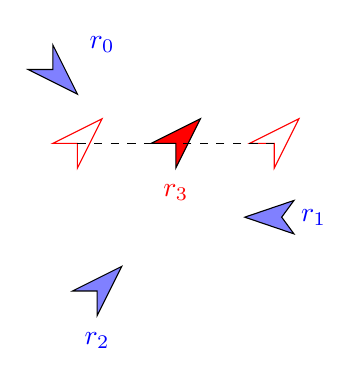
\begin{tikzpicture}[scale=1.25]
      \draw[fill=blue!50] (3.2,2.5) -- (2.95,2.5) -- (3.45,2.75) -- (3.2,2.25)   -- cycle;
      \node[color=blue] at (3.2, 2) {$r_2$};
      % draw grids
      % \draw[color=gray, help lines, line width=.05pt] (-1,1)  grid[xstep=.5cm, ystep=.5cm] (6,6);
      \draw[fill=blue!50] (3,4.5) -- (2.75,5) -- (2.75,4.75) -- (2.5,4.75)   -- cycle;
      \node[color=blue] at (3.25, 5) {$r_0$};
      \draw[fill=blue!50] (5.2,3.42) -- (4.7,3.25) -- (5.2,3.08) -- (5.075,3.25)  -- cycle;
      \node[color=blue] at (5.4,3.25) {$r_1$};    
      \draw[fill=red] (4,4) -- (3.75,4) -- (4.25,4.25) -- (4,3.75) -- cycle;
      \node[color=red] at (4, 3.5) {$r_3$};
      \draw[color=red] (3,4) -- (2.75,4) -- (3.25,4.25) -- (3,3.75) -- cycle;
      \draw[dashed] (3,4) -- (4,4);
      % \draw (0,-4.75) node[below] {reflect across $x$-axis};  
      \draw[color=red] (5,4) -- (4.75,4) -- (5.25,4.25) -- (5,3.75) -- cycle;
      \draw[dashed] (5,4) -- (4,4);
    \end{tikzpicture}
  \end{minipage}
  \begin{minipage}[b]{0.45\linewidth}
    \centering
    \begin{tikzpicture}[scale=1.25]
      \node[] (A) at (4,4)    {$\langle3\rangle$};
      \node[] (B) at (3,2.5)  {$\langle2\rangle$};
      \node[] (C) at (5.5,4)  {$\langle3,1\rangle$};
      \node[] (D) at (3,5)    {$\langle3,0\rangle$};
      \draw[edge] (A) -- (D);
      \draw[edge] (A) -- (C);
    \end{tikzpicture}
  \end{minipage}
  \caption{[left] A root robot $r_3$ has three neighbors, and two outgoing
  edges from its role vertex.  [right] After exchanging messages. Robot $r_3$ selects $r_0$ and $r_1$ as its children since they are two robots who are closest to two desired opening position corresponding to the out-edges. Robot $r_2$ is an orphan without any assignment.}
  \label{fig:authtree}
\end{figure}
%%%%%%%%%%%%%%%%%%%%%%%%%%%%%%%%%%%%%%%%

%\clearpage
\section{Distributed Task-Assignment}
\label{sec:task-assgin-algo}

In this section we describe the primary version of our formation algorithm. 
%
The algorithm takes the lattice graph as input to form the desired lattice pattern. 
%
Generally each robot repeats following steps every $\dt$ seconds:
\begin{enumerate}
\item Step 1: robots use the matching contained in received messages to
  construct an authority tree based on their IDs.
\item Step 2: each robot decides its ``role'', which is essentially a        vertex in the lattice graph, it is supposed to play in the formation.  
    %
    The root of the authority tree selects the first vertex in the lattice graph as its role; 
    the descendant robots in the authority tree accept their roles as part of the task assignment from their parents. 
\item Step 3: each robot finds a position, if any, where no robot is         assigned and located, as the opening position it knows.
\item Step 4: each robot computes several destinations in its body frame to
  assign its matching neighbors, using the standard Hungarian
  algorithm~\cite{Kuh55}. 
  %
  Each robot broadcasts a message containing its assignment, along with the authority value, and the opening position, if any, to its neighbors.
\item Step 5: each robot computes its destination based on the assigned task and  moves toward to the assigned destination according the motion strategy discussed in part~\ref{sec:motion}.
\end{enumerate}

\subsection{Task Assignment}
\label{subsec:task}


Once the authority tree is constructed, each root robot selects the first vertex of the lattice graph as its role; the descendant robot accepts a role from its parent.

For a robot $r_i$ who already selects its role, it needs to establish a
relationship, called \textbf{matching} between its neighbors and the outgoing edges from its role vertex. 
\begin{defn}
\label{def:matching}
  Given a robot $r_i$ and a role vertex $v$ for that robot, let the lattice
  graph edge set
    $E=\{\emptyset, e_{v}^w, e_{v}^u, \ldots\}$
  be the set that contains a null value $\emptyset$ and all outgoing edges from vertex $v$.  
  Let
    $I=\{\id_a, \id_b, \ldots \}$
  be the set that contains the IDs of the neighbors of $r_i$.  
  Then a
  \textbf{matching for $r_i$} is a function $g : I \rightarrow E$ that
  associates each neighbor ID with either a lattice graph edge from its role vertex or with the null value.
\end{defn}
For example, in Figure~\ref{fig:authtree}, robot $r_2$ is an orphan robot to the root robot $r_3$, with $g(\id_{r_2}) = \emptyset$.

Assume robot $r_i$ has $N_i$ neighbors and its outdegree is $E_i$. 
%
We interpret this problem as a task assignment problem~\cite{Kuh55, Mun57}: given $\min(N_i, E_i)$ agents and $E_i$ tasks, we create a $\min(N_i, E_i)\times E_i$ matrix containing the cost of assigning each agent to a task. 
%
The goal is finding the cost minimizing assignment. 
%
(The number of agents is not greater than the number of
the out-degree since a parent robot always selects maximum $E_i$ neighbors as to form matching with it).

Specifically, in the cost matrix, each row corresponds to an ID of a non-orphan neighbor of $r_i$, and each column corresponds to an out-edge from its role $f(r_i)$. 
%
The cost is defined as the Euclidean distance for a neighbor robot to
travel from its current position $(x^{(i)}, y^{(i)})$ to the desired
position $(\bar{x}^{(i)}, \bar{y}^{(j)})$. 
%
%TODO: replace transformation T with \math font, consistent with RAL
Given an edge $e$, we can use its transformation $\Tr(e)$ to find the desired position.
\begin{equation}
  \label{eq:trans-pos}
  \left[\bar{x}^{(i)} \quad \bar{y}^{(i)} \quad 1\right]^\top = \Tr(e) \left[0 \quad 0 \quad 1\right]^\top
\end{equation}

The procedure to construct the cost matrices for a root robot and a descendant robot are slightly different.

\subsubsection{Root Matching}


For a root robot $r_i$, in its cost matrix of 
\begin{enumerate}
  \item Each row of the matrix corresponds to a neighbor of $r_i$;
  \item Each column of the matrix corresponds to an out-edge of $f(r_i)$;
  \item The entry of the matrix in row $j, j \in [1, \min(N_i, E_i)]$, column
    $k, k \in (1, E_i)$ represents the Euclidean distance $|| \bar{p}_j^{(i)} -
    {p}_j^{(i)} ||$ between the current position of the $j^{th}$ neighbor and
    its desired position if matched with the $k^{th}$ outgoing edge (both computed in the body frame of $r_i$).  
\end{enumerate}

We apply the Hungarian Algorithm~\cite{Kuh55} to solve the assignment problem in polynomial time. 
%
Each robot executes the Hungarian algorithm on the cost matrix
to compute matching of its neighbors to its outgoing edges, by minimizing the total Euclidean distance. 
%
The algorithm takes $O(N_i^3)$ time complexity.

%
The center robot, which is a root, finds matching for four of its
neighbors and assign them to desired poses in its body frame, meanwhile, there
is no matching found for one of its neighbors.
%%%%%%%%%%%%%%%%%%%%%%%%%%%%%%%%%%%%%%%%%%%%%%
\begin{figure}
    \centering
    \begin{minipage}{0.9\textwidth}
    \centering
      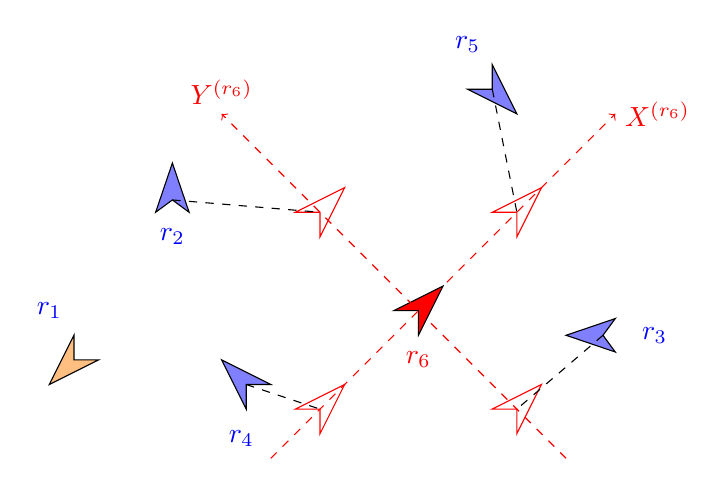
\begin{tikzpicture}[scale=1.25]
    \draw[fill=red] (3,3) -- (2.75,3) -- (3.25,3.25) -- (3,2.75) -- cycle;
    \node[color=red] at (3, 2.5) {$r_6$};
    %\draw[thick, ->] (-1,0) -- (6,0) node[right] {X};
    %\draw[thick, ->] (0,-1) -- (0,6) node[above] {Y};
    \draw[color=red, dashed, ->] (1.5,1.5) -- (5,5) node[right] {$X^{(r_6)}$};
    \draw[color=red, dashed, ->] (4.5,1.5) -- (1,5) node[above] {$Y^{(r_6)}$};
    % draw grids
    %\draw[color=gray, help lines, line width=.05pt] (-1,1)  grid[xstep=.5cm, ystep=.5cm] (6,6);
    \draw[fill=blue!50] (0.5,4.5) -- (0.33,4) -- (0.5,4.125) -- (0.67,4)    -- cycle;
    \node[color=blue] at (0.5,3.75) {$r_2$};
    \draw[fill=blue!50] (4,5) -- (3.75,5.5) -- (3.75,5.25) -- (3.5,5.25)        -- cycle;
    \node[color=blue] at (3.5,5.7) {$r_5$};
    \draw[fill=blue!50] (1,2.5) -- (1.25,2) -- (1.25,2.25) -- (1.5,2.25)        -- cycle;
    \node[color=blue] at (1.2,1.7) {$r_4$};
    \draw[fill=blue!50] (5,2.92) -- (4.5,2.75) -- (5,2.58) -- (4.875,2.75)  -- cycle;
    \node[color=blue] at (5.4,2.75) {$r_3$};
%    \draw[fill=blue!50] (2.5,0) -- (2.7,0.52) -- (2.5,0.35) -- (2.3,0.52)   -- cycle;
%    \node[color=blue] at (2.5,0.75) {$r_1$};
    \draw[fill=orange!50] (-0.5,2.5) -- (-0.5,2.75) -- (-0.75,2.25) -- (-0.25,2.5)  -- cycle;
    \node[color=blue] at (-0.75,3) {$r_1$};
        
    \draw[color=red] (4,4) -- (3.75,4) -- (4.25,4.25) -- (4,3.75) -- cycle;
    \draw[color=red] (2,2) -- (1.75,2) -- (2.25,2.25) -- (2,1.75) -- cycle;
    \draw[color=red] (2,4) -- (1.75,4) -- (2.25,4.25) -- (2,3.75) -- cycle;
    \draw[color=red] (4,2) -- (3.75,2) -- (4.25,2.25) -- (4,1.75) -- cycle;
        
    \draw[dashed](0.5, 4.125) -- (2,4);
    \draw[dashed](1.25,2.25) -- (2,2);
    \draw[dashed](3.75,5.25) -- (4,4);
    \draw[dashed](4.875,2.75) -- (4,2);
%   \draw (0,-4.75) node[below] {reflect across $x$-axis};  
  \end{tikzpicture}
    \end{minipage}
    \caption{Matching computed by the root robot $r_6$.}
    \label{fig:formsquare}
\end{figure}
%%%%%%%%%%%%%%%%%%%%%%%%%%%%%%%%%%%%%%%%%%%%%
\begin{figure}
    \centering
    \begin{tikzpicture}[scale=1.5]
    \node[] (I) at (3,3)   {$\langle6\rangle$};
    \node[] (B) at (0,2)   {$\langle6,4,1\rangle$};
    \node[] (C) at (2,4)   {$\langle6,2\rangle$};
    \node[] (D) at (4,2)   {$\langle6,3\rangle$};
    \node[] (E) at (2,2)   {$\langle6,4\rangle$};
    \node[] (F) at (4,4)   {$\langle6,5\rangle$};
    
    \draw[edge] (I) -- (C);
    \draw[edge] (I) -- (D);
    \draw[edge] (I) -- (E);
    \draw[edge] (I) -- (F);
    \draw[edge] (E) -- (B);
\end{tikzpicture}
\caption{Authority tree constructed by the robots in Figure~\ref{fig:formsquare}.}
    \label{fig:formsquare-auth}
\end{figure}
%%%%%%%%%%%%%%%%%%%%%%%%%%%%%%%%%%%%%%%%%%%%%%

\subsubsection{Descendant Matching}

Similar to the process of computing matching for the root robot, the steps to compute matching for a descendant robot are identical except for two differences:
\begin{enumerate}
\item A descendant robot chooses its role according to the matching received from its parent.  
%
    Specifically, the role of a descendant is the terminal vertex of
  the edge associated with its own ID in that matching. 
\item A descendant robot, in its matching, ensures that the parent is
  matched with one of its outgoing edges, whose transformation is the inverse of the edge matching it.
\end{enumerate}

Figure~\ref{fig:formsquare} shows the procedure of computing the matching by a root robot and a descendant robot, respectively. 
%
Assume a square lattice graph in Figure~\ref{fig:sq} is given, robot $r_6$ has $5$ neighbors $r_1, r_2, r_3, r_4, r_5$;
robot $r_4$ has three neighbors $r_6, r_2, r_1$. 
%
By exchanging messages, the authority tree constructed by the robots is shown in Figure~\ref{fig:formsquare-auth}.
%
Then $r_6$ is a root and it chooses the first vertex of the lattice graph as its role.
%
The root robot $r_6$ computes four desired positions in its body frame according to the cost matrix for its descendants.
%
Robot $r_1$ is too far away to be selected by $r_6$ to form matching, so it is an orphan (Figure~\ref{fig:formsquare}).
%
On the other side, robot $r_4$ recognizes itself as a descendant of the root $r_6$.
%
It first computes its own matching for its neighbors, $r_6,r_2, r_1$, in its local frame. 
%
However, $r_4$ must force its matching with $r_6$ to be consistent with $r_6$'s matching with it.
%
Recall that $r_6$ already assigns a role vertex to $r_4$, which corresponds to the position behind the root $r_6$ (the red hollow arrow in Figure~\ref{fig:formsquare-des}).
%
Therefore, $r_4$ finds the reverse edge with a terminal node matching that destination in its own frame, that is, the position in front of its head. 
%
Then it matches the root to this edge with itself and compute the local optimal matching for the rest of its neighbors $r_2, r_1$.

%%%%%%%%%%%%%%%%%%%%%%%%%%%%%%%%%%%%%%%%%%%%%%
\begin{figure}
    \centering
    \begin{minipage}{0.9\textwidth}
    \centering
    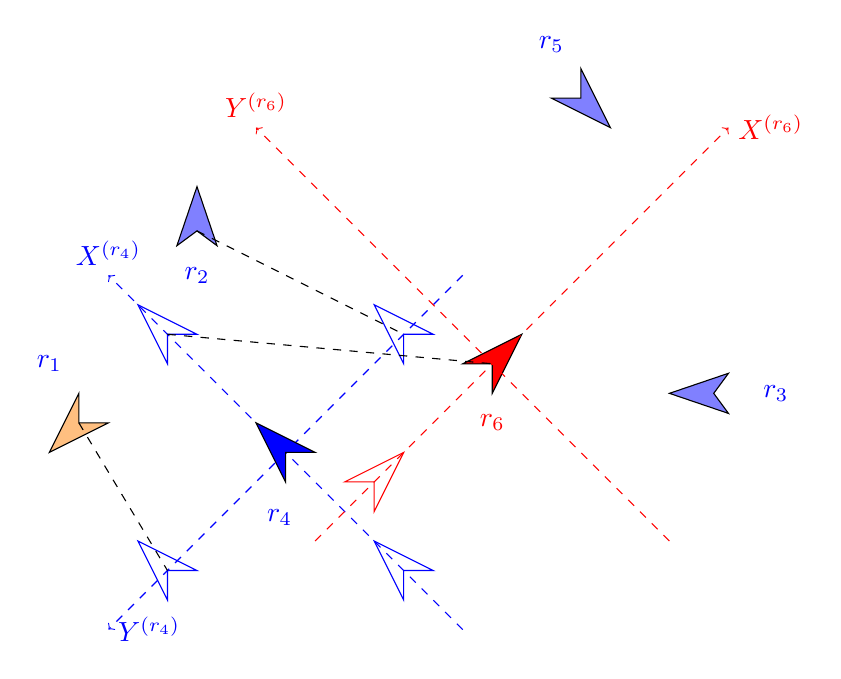
\begin{tikzpicture}[scale=1.5]
    \draw[fill=red] (3,3) -- (2.75,3) -- (3.25,3.25) -- (3,2.75)        -- cycle;
    \node[color=red] at (3, 2.5) {$r_6$};
    %\draw[thick, ->] (-1,0) -- (6,0) node[right] {X};
    %\draw[thick, ->] (0,-1) -- (0,6) node[above] {Y};
    % draw grids
    %\draw[color=gray, help lines, line width=.05pt] (-1,1)  grid[xstep=.5cm, ystep=.5cm] (6,6);
    % center of rc : 0.5, 4.125
    \def\Cx{0.5}
    \def\Cy{4.125}
    \def\d{1.5}
    \def\dd{1}
    \coordinate (C) at (\Cx, \Cy);
    \def\Ex{1.25}
    \def\Ey{2.25}
    \coordinate (E) at (\Ex, \Ey);
    \draw[color=blue, dashed, ->] (\Ex+\d, \Ey+\d) -- (\Ex-\d,\Ey -\d) node[right] {$Y^{(r_4)}$};
    \draw[color=blue, dashed, ->] (\Ex +\d,\Ey-\d) -- (\Ex -\d,\Ey+\d) node[above] {$X^{(r_4)}$};
    \draw[fill=blue!50] (0.5,4.5) -- (0.33,4) -- (C) -- (0.67,4) -- cycle;
    \node[color=blue] at (0.5,3.75) {$r_2$};
    \draw[fill=blue!50] (4,5) -- (3.75,5.5) -- (3.75,5.25) -- (3.5,5.25)  -- cycle;
    \node[color=blue] at (3.5,5.7) {$r_5$};
    \draw[fill=blue] (1,2.5) -- (1.25,2) -- (E) -- (1.5,2.25)  -- cycle;
    \node[color=blue] at (1.2,1.7) {$r_4$};
    \draw[fill=blue!50] (5,2.92) -- (4.5,2.75) -- (5,2.58) -- (4.875,2.75)  -- cycle;
    \node[color=blue] at (5.4,2.75) {$r_3$};
    \draw[fill=orange!50] (-0.5,2.5) -- (-0.5,2.75) -- (-0.75,2.25) -- (-0.25,2.5)  -- cycle;
    \node[color=blue] at (-0.75,3) {$r_1$};
    \coordinate (I) at (3,3);
    \coordinate (B) at (-0.5, 2.5);
    \draw[color=blue] (1-\dd,2.5+\dd) -- (1.25-\dd,2+\dd) -- (\Ex-\dd, \Ey+\dd) -- (1.5-\dd,2.25+\dd)  -- cycle;
    \draw[color=blue] (1-\dd,2.5-\dd) -- (1.25-\dd,2-\dd) -- (\Ex-\dd,\Ey-\dd) -- (1.5-\dd,2.25-\dd)  -- cycle;
    \draw[color=blue] (1+\dd,2.5-\dd) -- (1.25+\dd,2-\dd) -- (\Ex+\dd, \Ey-\dd) -- (1.5+\dd,2.25-\dd)  -- cycle;
    \draw[color=blue] (1+\dd,2.5+\dd) -- (1.25+\dd,2+\dd) -- (\Ex+\dd,\Ey+\dd) -- (1.5+\dd,2.25+\dd)  -- cycle;
    
    \draw[color=red, dashed, ->] (1.5,1.5) -- (5,5) node[right] {$X^{(r_6)}$};
    \draw[color=red, dashed, ->] (4.5,1.5) -- (1,5) node[above] {$Y^{(r_6)}$};
    \draw[dashed](C) -- (\Ex+\dd, \Ey+\dd);
    \draw[dashed](B) -- (\Ex-\dd, \Ey-\dd);
    
    \draw[color=red] (2,2) -- (1.75,2) -- (2.25,2.25) -- (2,1.75) -- cycle;
    \draw[dashed](\Ex-\dd, \Ey+\dd) -- (I);
\end{tikzpicture}
    \end{minipage}
    \caption{Matching computed by the descendant robot $r_4$.}
    \label{fig:formsquare-des}
\end{figure}
%%%%%%%%%%%%%%%%%%%%%%%%%%%%%%%%%%%%%%%%%%%%%%

%\clearpage
\section{Motion Strategy}
\label{sec:motion}

Each robot determines its destination at the final step of the algorithm.  
%
We apply different moving plans for robots of different status:
\begin{enumerate}
\item Root -- the robot who has the highest authority among neighbors -- does not move;
\item Descendant -- the robot who has a neighbor with higher authority and has matching with it -- moves toward assigned destination subject to Lemma~\ref{lem:boundedrange};
\item Orphan -- the robot whose neighbors' authorities are higher but have no task assigned to it -- moves away from its current ``parent''.
\end{enumerate} 


We assume that the robot can rotate extremely fast, and provide a lemma to ensure the descendant robot remain in the range of its parent during its movement. 

Figure~\ref{fig:boundedrange} shows an example in which the actual
pose $p_p(t+\dt)$ of parent robot $r_p$ could be anywhere in the dotted
circle. 
%
The desired pose $\bar{p}_i^{(p)}(t)$ for $r_i$ is assigned by $r_p$ at
time $t$.  
%
On the boundary of the intersection of $P_p \cap P_i$ (shaded area),
the nearest point to the desired ultimate destination position is
selected as the real destination position for $r_i$ at time $t+\dt$.

\begin{lem}
  \label{lem:boundedrange}
  If robot $r_i$ is the neighbor of robot $r_p$ at time $t$, it will still be the 
  neighbor of $r_p$ at time $t + \dt$ if $|| p_i(t+\dt) - p_p(t) || \leq \range -  v\dt$, where $v$ is the velocity of $r_i$ and $r_p$. 
\end{lem}

\begin{proof}
Because $r_i$ and $r_p$ are initially neighbors, we have
  \begin{equation}
    || p_i(t) - p_p(t) || \leq \range.
  \end{equation}
Due to the velocity limits on the robots, we also know that
  \begin{equation}\label{eq:d1}
    || p_p(t+\dt)- p_p(t) ||\leq v\dt.
  \end{equation}
since we assume that 
  \begin{equation}\label{eq:d2}
    || p_p(t) - p_i(t+\dt) || \leq \range - v\dt
  \end{equation}
then applying triangle inequality to Equation~\ref{eq:d1} and Equation~\ref{eq:d2} yields
  \begin{eqnarray*}
  \label{eq:d3}
    || p_p(t+\dt) - p_i(t+\dt) || & \leq || p_p(t+\dt) - p_i(t)|| \\
      & + || p_i(t) - p_i(t+\dt)|| \\
      & \leq \range - v\dt + v\dt = \range
  \end{eqnarray*}
\end{proof}
\begin{figure}
    \centering
      \def\firstcircle{(0,0) circle (2cm)}
  \def\secondcircle{(2.3,1.8) circle (1.5cm)}
  \def\thirdcircle{(0,0) circle (1.5cm)}
  \colorlet{circle edge}{blue!50}
  \colorlet{circle area}{blue!20}
  \tikzset{filled/.style={fill=circle area, draw=circle edge, thick},
    outline/.style={draw=circle edge, thick}}
  \tikzstyle{important line}=[very thick]
  \centering
  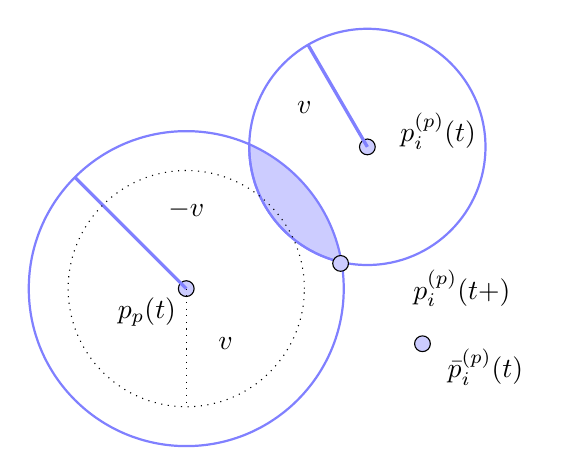
\begin{tikzpicture}
    \begin{scope}
        \clip \firstcircle;
        \fill[filled] \secondcircle;
    \end{scope}
    \draw[outline] \firstcircle node {$ $};
    \draw[fill=circle area] (0,0) circle (0.1cm); 
    \node at (-0.5,-0.3) {$p_p(t)$};
    \draw[style=important line, circle edge](90:1cm) -- node[black]{$\range- v\dt$}+(0,0);
   \draw[style=important line, circle edge](0,0) -- (135:2cm);
    \draw[outline] \secondcircle node {$ $};

    \draw[fill=circle area] (2.3,1.8) circle (0.1cm); 
    \node at (3.2, 2) {$p_i^{(p)}(t)$};

   \draw[style=important line, circle edge](2.3, 1.8) -- (1.55,3.09);
   \node at (1.5, 2.3) {$v\dt$};

    \draw[fill=circle area] (3, -0.7) circle (0.1cm); 
    \node at (3.8,-1) {$\bar{p}_i^{(p)}(t)$};
    \draw[dotted] \thirdcircle node{$ $};

   \draw[dotted](0, 0) -- (0,-1.5);
   \node at (0.5, -0.7) {$v\dt$};

  \draw[fill=circle area] (1.96, 0.32) circle (0.1cm); 
    \node at (3.5,0) {${p}_i^{(p)}(t+\dt)$};
  \end{tikzpicture}
  \caption{The real destination for the descendant robot $r_i$ to maintain connected with its parent $r_p$ during time $t+\dt$.}
    \label{fig:boundedrange}
\end{figure}

Lemma~\ref{lem:boundedrange} guarantees that a descendant robot always connects with its parent. 

Recall that an orphan robot is a special descendant who does not have an actual task assigned by its parent's matching, our motion plan simply drives the orphan robot away from its ``parent''. 
%
In detail, if the orphan robot receives a message from its parent, in which it is matched to $\emptyset$, it concludes that its current location is too congested with robots around.
%
In response, it moves directly away from its parent for a fixed period of time, equal to $2\range/v$.
%
During this time, it does not communicate with anyone, and is neither root nor descendant. 
%
When this time expires, the robot resumes normal execution. 
%
The effect is to disperse the robots without oscillations, which could occur when the robot selects a new parent immediately afterward.
 

%\clearpage
\section{Experiments}
\label{sec:mrf-exp}
We have demonstrated the effectiveness of our algorithm using simulations implemented with C++. 
%
Recall that Figure~\ref{fig:octsq-init-final} shows a simulation result of forming the repeating octagon-square lattice pattern with $100$ robots.
%
The acknowledgement to Liu is addressed for his open-source contribution of the Hungarian algorithm implementation~\cite{LiuShe11, LiuShe12a}.


We conduct experiments in an obstacle-free environment to measure the algorithm execution time (the units of measurement are the simulation steps) and final lattice formation quality. 
%
Three types of repeating lattice patterns: hexagon (Figure~\ref{fig:hex}), square (Figure~\ref{fig:sq}), and octagon-square (Figure~\ref{fig:octagonsquare}) are used to test our algorithm.
%
For each lattice pattern, we perform a series of experiments. 
%
In all experiments we vary the number of robots $n$ between $50$ and $250$ in increments of $50$.  
%
For each $n$, $50$ trials of experiments are tested with uniform distributions of initial poses randomly generated given distinct random seeds.

Figures~\ref{fig:octagonsquare-init-final}, \ref{fig:hex-init-final} and \ref{fig:sq-init-final} shows simulation results of three trials of experiments. 
%
In Figure~\ref{fig:octagonsquare-init-final}, the experiment took $\Time=1138$ simulation steps for $100$ robots to form a repeating octagon-square lattice pattern, with the fulfillment ratio $\Quality=0.694$.
% 
In Figure~\ref{fig:hex-init-final}, the experiment took $\Time=892$ simulation steps for $150$ robots to reach positions composing a repeating hexagon lattice pattern, with $\Quality=0.819$.
%
In Figure~\ref{fig:sq-init-final}, the experiment took $\Time=910$ simulation steps to form a repeating square pattern with $200$ robots, and the final fulfillment ratio $\Quality=0.725$.

%%%%%%%%%%%%%%%%%%%%%%%%%%%%%%%%%%%%%%%%
\begin{figure}
    \centering
   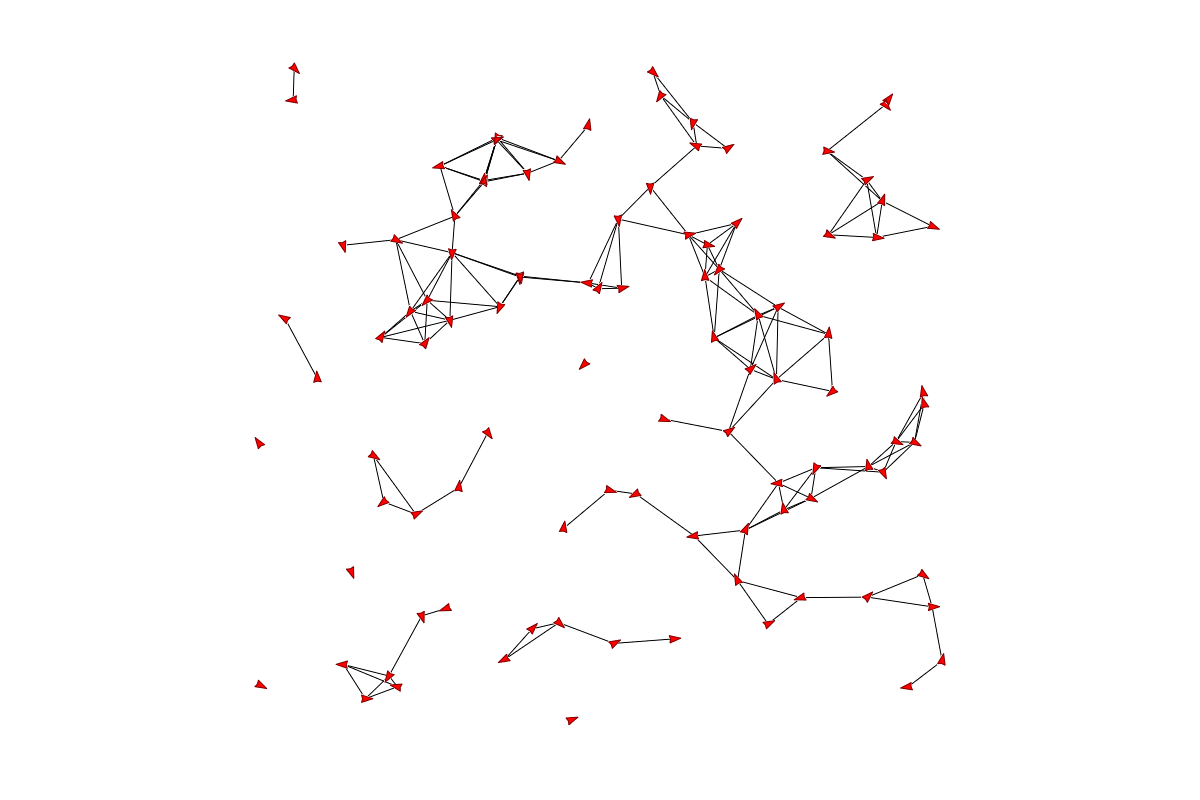
\includegraphics[trim=5cm 0cm 5cm 0cm, clip=true, width=0.8\textwidth]{figs/octsq100_init.png}
   \bigskip
   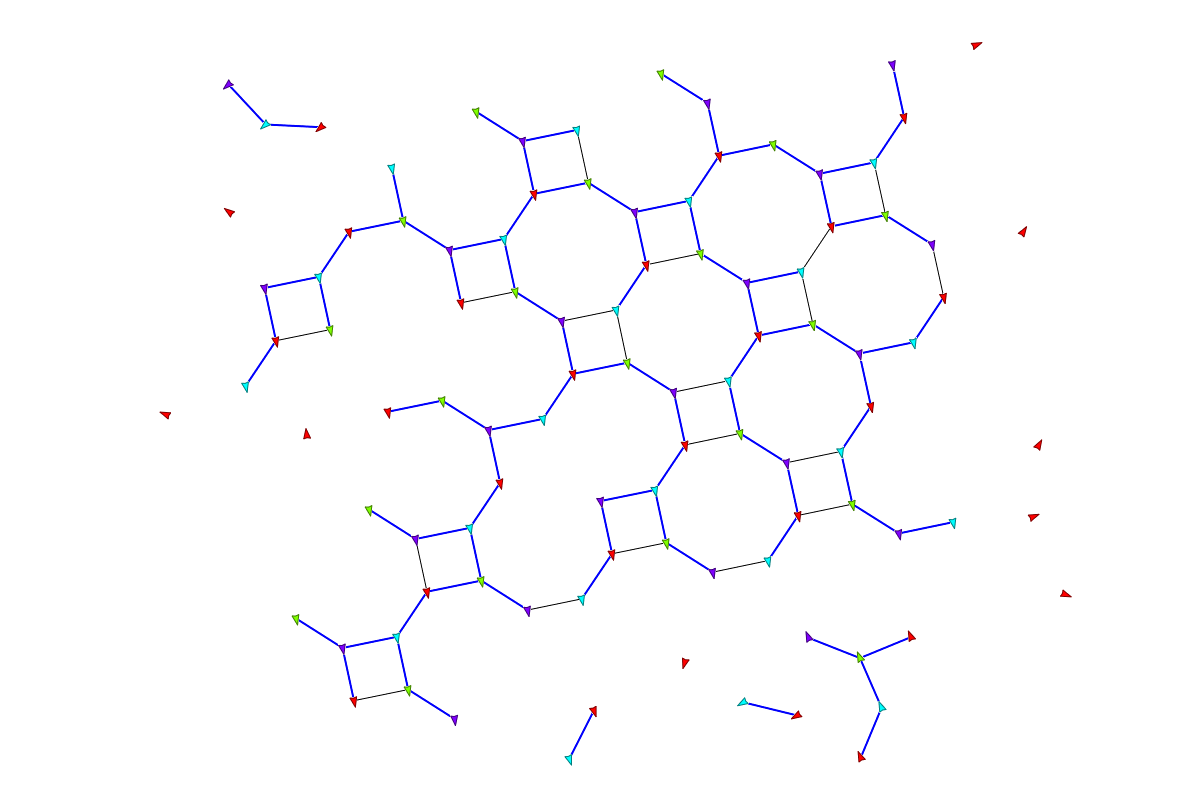
\includegraphics[trim=5cm 0cm 5cm 0cm, clip=true, width=0.8\textwidth]{figs/octsq100_final.png}
   \caption{[top] The initial poses of $100$ robots. [bottom] The final repeating hexagon pattern.}
   \label{fig:octagonsquare-init-final}
\end{figure}

%%%%%%%%%%%%%%%%%%%%%%%%%%%%%%%%%%%%%%%%
\begin{figure}
    \centering
  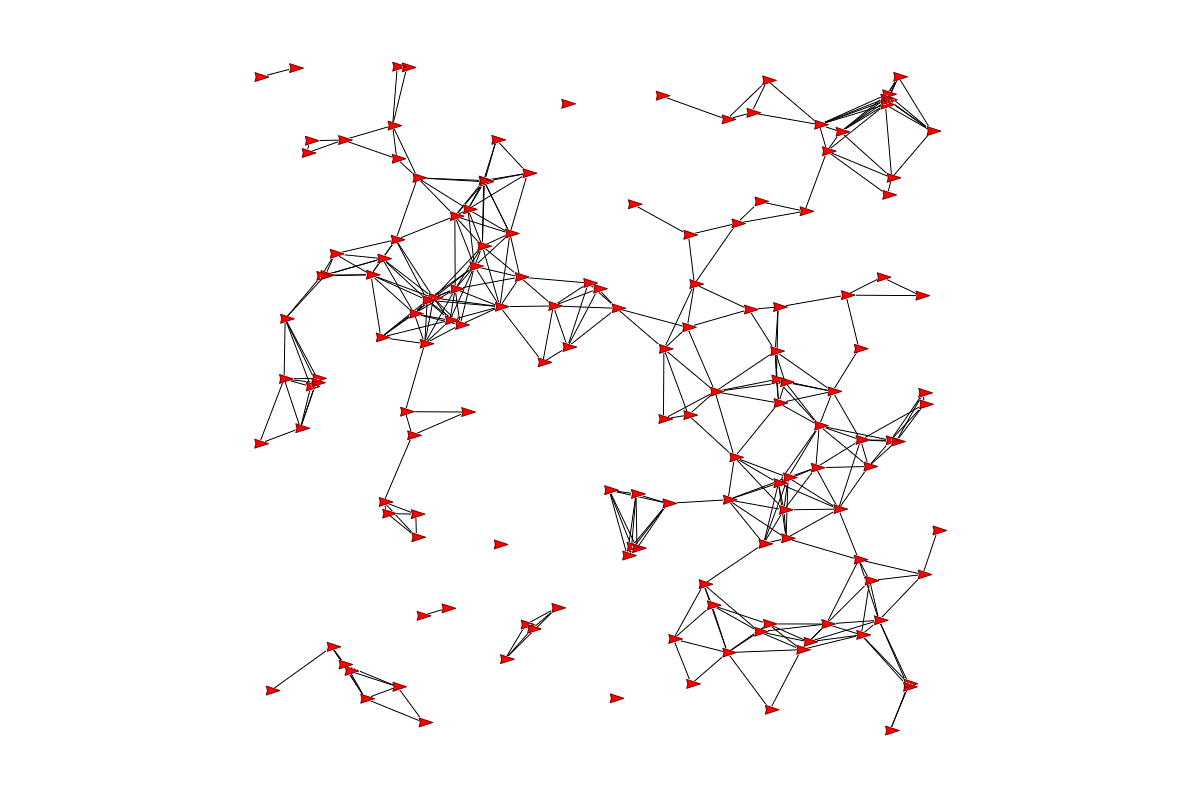
\includegraphics[trim=5cm 0cm 5cm 0cm, clip=true, width=0.8\textwidth]{figs/hex150_init.png}
  \bigskip
  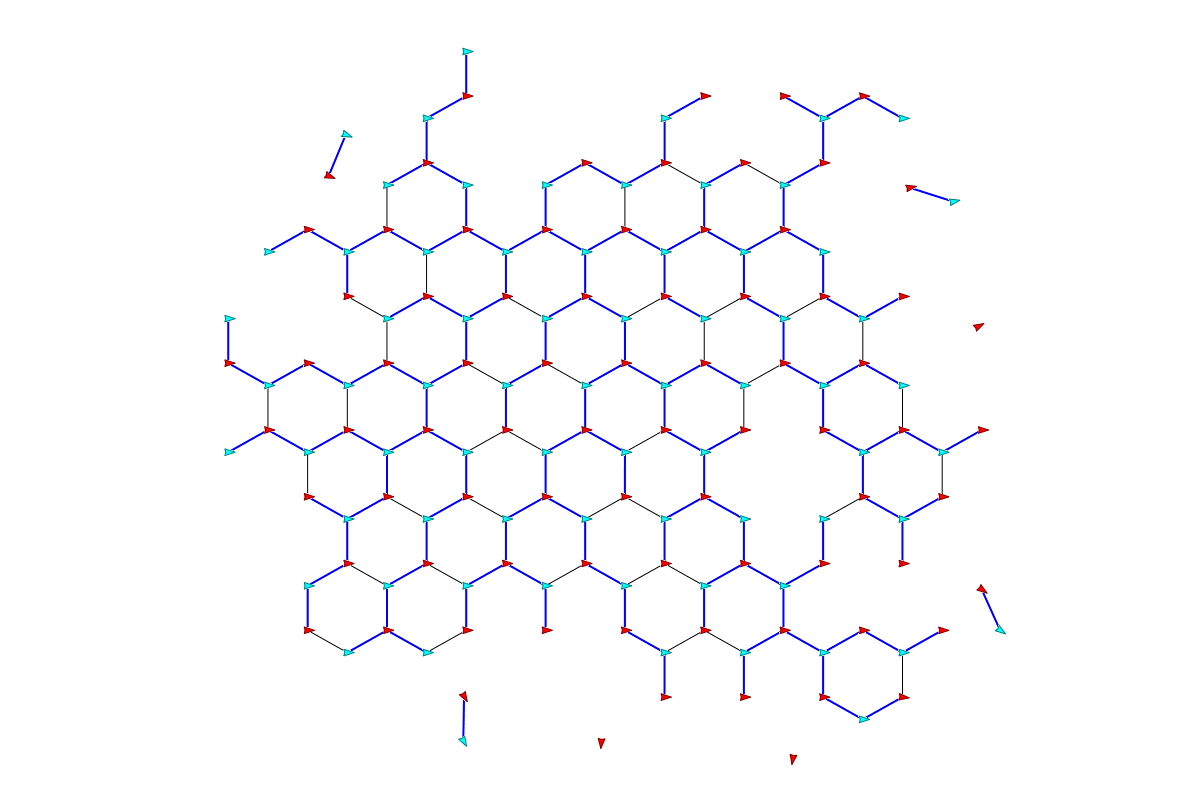
\includegraphics[trim=5cm 0cm 5cm 0cm, clip=true, width=0.8\textwidth]{figs/hex150_final.png}
  \caption{[top] The initial poses of $150$ robots. [bottom] The final repeating hexagon pattern.}
  \label{fig:hex-init-final}
\end{figure}


%%%%%%%%%%%%%%%%%%%%%%%%%%%%%%%%%%%%%%%%
\begin{figure}
    \centering
  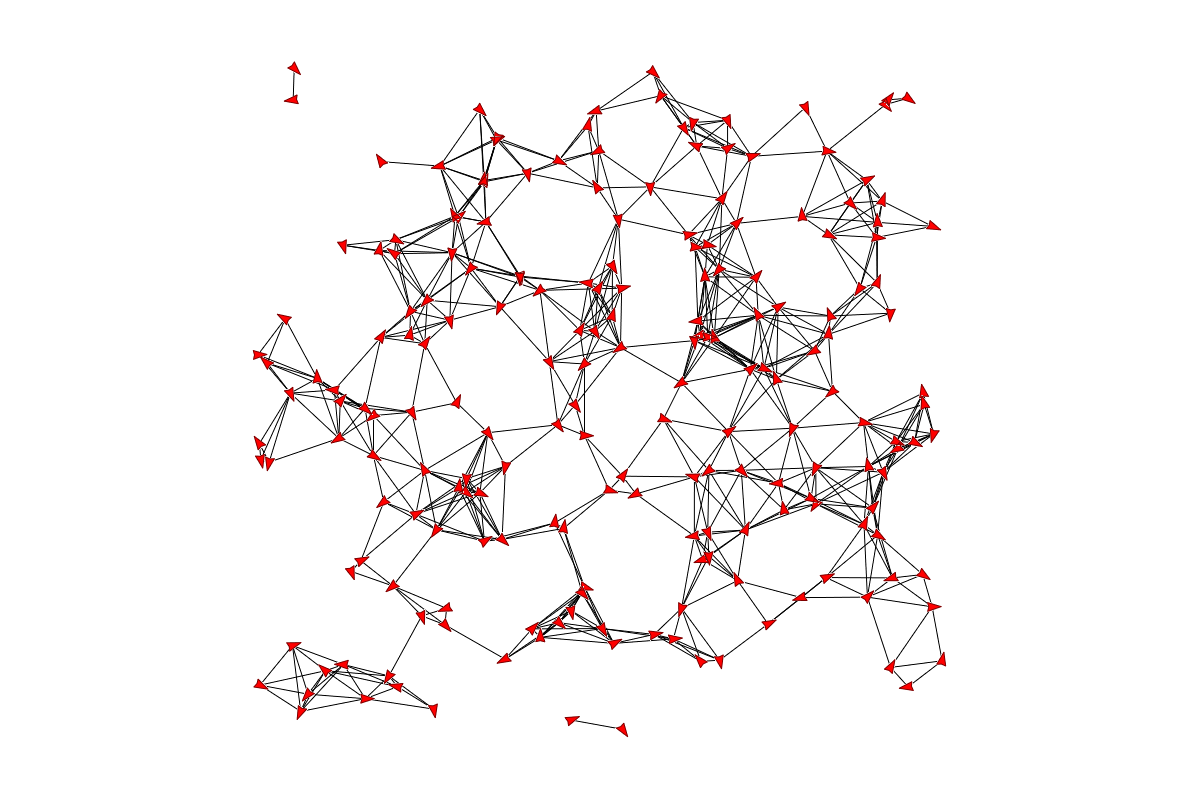
\includegraphics[trim=5cm 0cm 5cm 0cm, clip=true, width=0.8\textwidth]{figs/sq200_init.png}
  \bigskip
  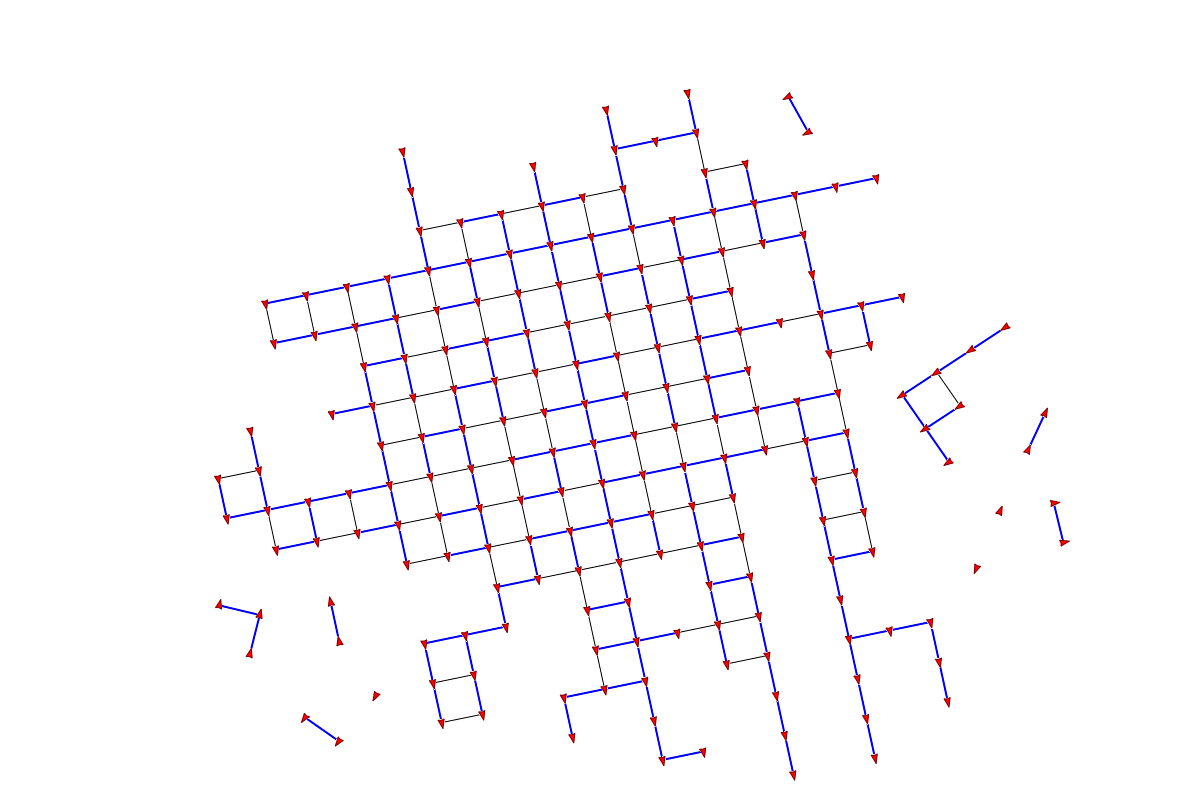
\includegraphics[trim=5cm 0cm 5cm 0cm, clip=true, width=0.8\textwidth]{figs/sq200_final.png}
  \caption{[top] The initial poses of $200$ robots. [bottom] The final repeating square pattern.}
  \label{fig:sq-init-final}
\end{figure}

We conclude from Figure~\ref{fig:exp-time} that the execution time scales reasonably with the increase of the number of robots, across all three given lattice graphs. 

%%%%%%%%%%%%%%%%%%%%%%%%%%%%%%%%%%%%%%%%
\begin{figure}
    \centering
   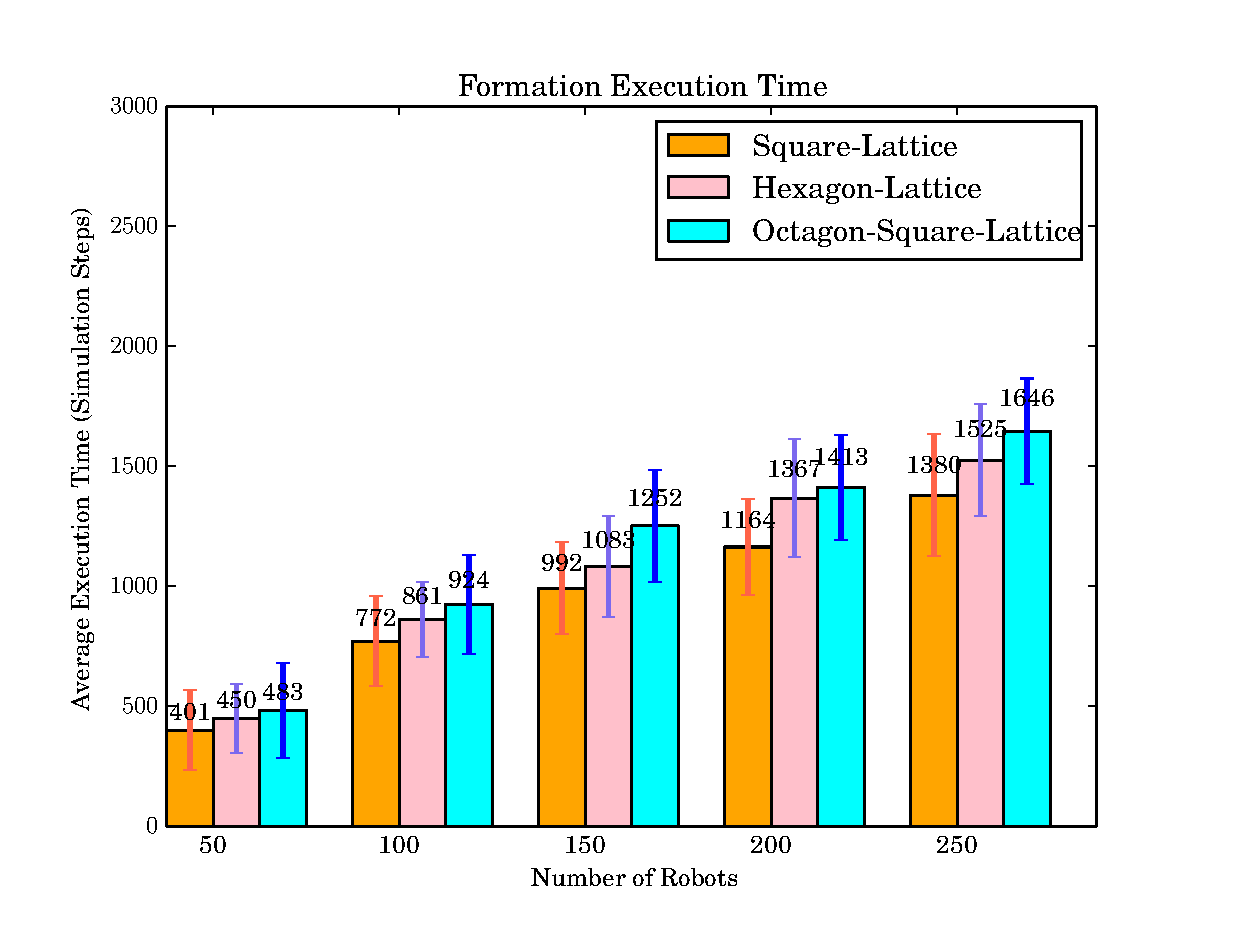
\includegraphics[width=\textwidth]{figs/exp_time}
    \caption{Average execution time and its standard deviation of forming repeated lattice patterns of square, hexagon and octagon-square.} 
    \label{fig:exp-time}
\end{figure}
%%%%%%%%%%%%%%%%%%%%%%%%%%%%%%%%%%%%%%%%

The initial distribution of robots' positions impacts the final formation quality in a certain sense.
%
Figure~\ref{fig:exp-qual} shows that when the number of robots is small and robots are sparsely distributed, most of robots do not have enough neighbors around, thus the average formation fulfillment ratio is less than the result from a denser distribution. 
%
Moreover, Figure~\ref{fig:exp-qual} shows a trend that the fulfillment ratio for
a repeated pattern increases as the number of robots increases and become closer to $1$.

%%%%%%%%%%%%%%%%%%%%%%%%%%%%%%%%%%%%%%%%
\begin{figure}
    \centering
   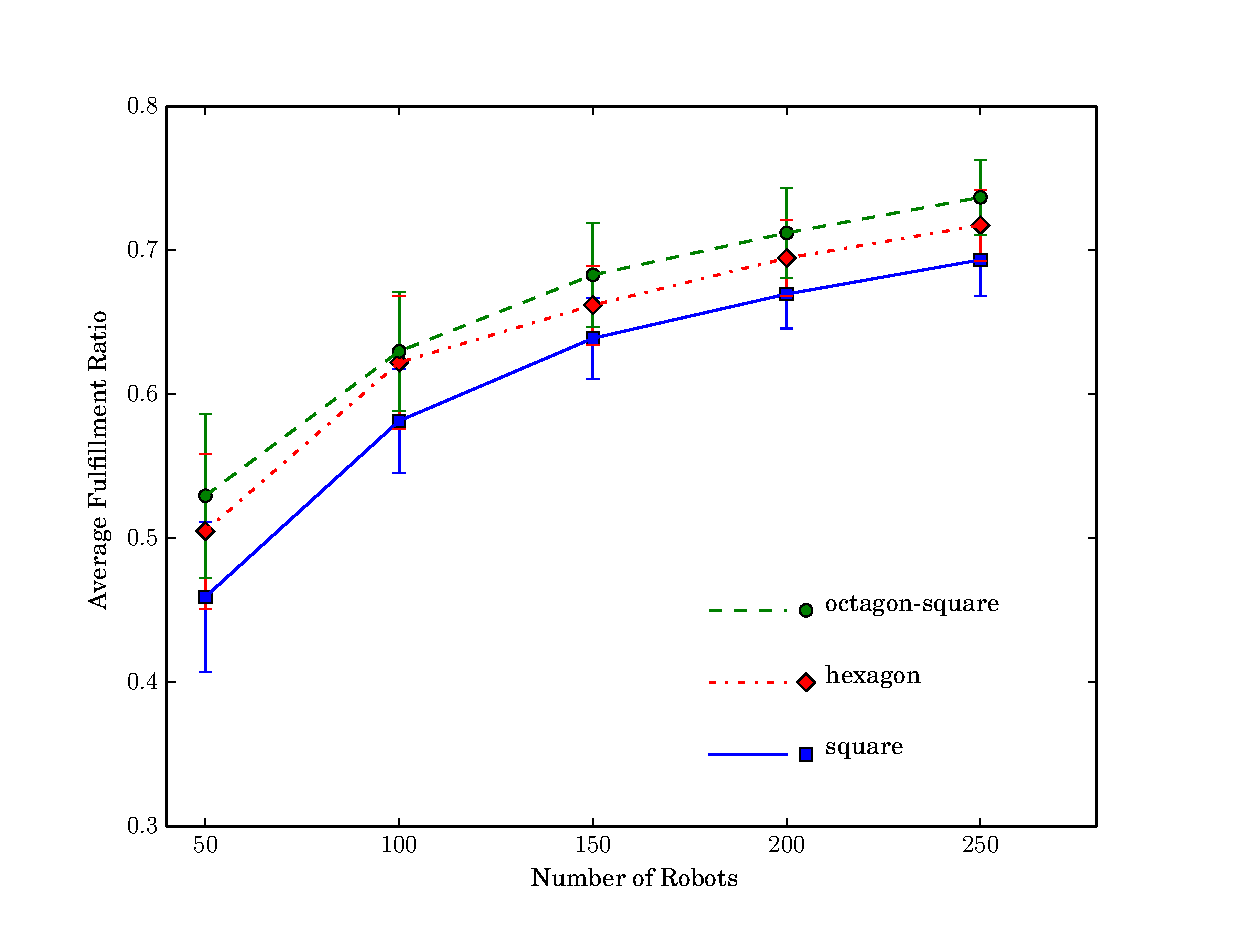
\includegraphics[width=\textwidth]{figs/exp_qual}
    \caption{Average fulfillment ratio and its standard deviation of forming lattice patterns of square, hexagon and octagon-square.} 
    \label{fig:exp-qual}
\end{figure}
%%%%%%%%%%%%%%%%%%%%%%%%%%%%%%%%%%%%%%%%


Additionally, we test the robustness of our algorithm with another set of experiments.
%
Figure~\ref{fig:robust} shows one test case in which some robots are removed from the system when the system reached the static state at the first time.
%
Initially, $150$ robots form a repeating hexagon pattern using the lattice graph (Figure~\ref{fig:hex}).  
%
It takes $1441$ simulation steps for all robots to reach static states, with final fulfillment ratio $\Quality=0.804$. 
%
After randomly removing $50$ robots, it takes another $1685$ simulation steps for robots to reach static states again, with the final fulfillment ratio $\Quality=0.713$. 
 %
Similar experiments are conducted and show that our algorithm works well after adding more robots to the system.

%%%%%%%%%%%%%%%%%%%%%%%%%%%%%%%%%%%%%%%%
\begin{figure}
    \begin{minipage}[b]{0.5\linewidth}
        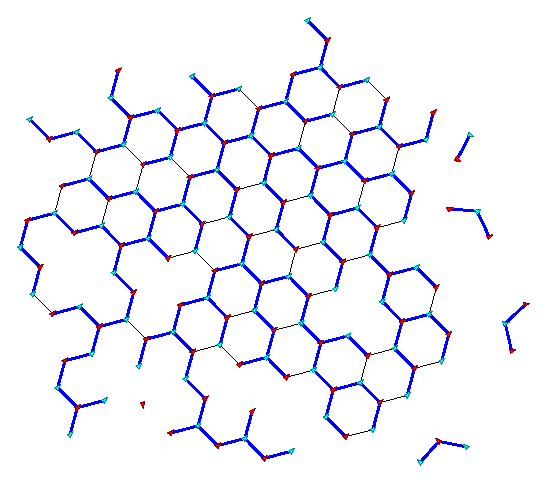
\includegraphics[width=.95\columnwidth]{figs/formation-150}
    \end{minipage}
    \begin{minipage}[b]{0.45\linewidth}
        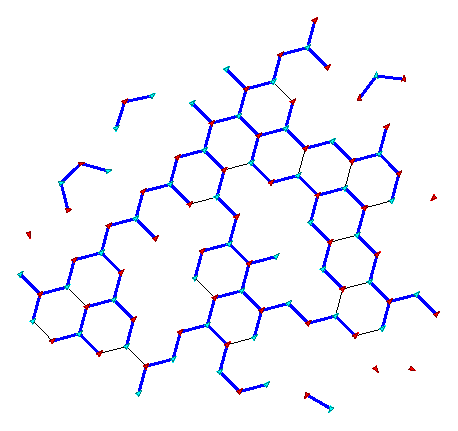
\includegraphics[width=.95\columnwidth]{figs/formation-100}
    \end{minipage}
    \caption{[left] The formation of repeated hexagon lattice with 150 robots. [right] The reconfigured formation after randomly removing 50 robots.}
\label{fig:robust}
\end{figure}
%%%%%%%%%%%%%%%%%%%%%%%%%%%%%%%%%%%%%%%%

Finally, we argue that our algorithm works well with non-repeating lattice patterns if we vary the problem assumptions.
%
For example, as shown in Figure~\ref{fig:p-letter}, in which five robots formed a ``P''
letter given a complete five-node lattice graph. 
%
In this case, additional constraints for are required: 
\begin{enumerate}
  \item The number of robots is the same as the number of vertices in the lattice graph.
  \item All robots are able to observe and communicate with each other initially.
\end{enumerate}
\begin{figure}
    \centering
  \begin{minipage}[b]{0.45\linewidth}
  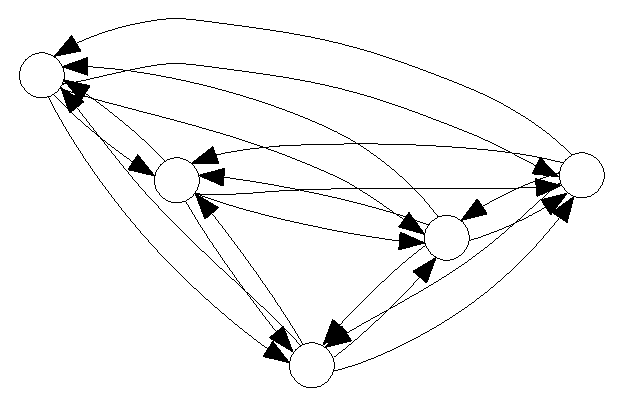
\includegraphics[width=.9\columnwidth]{figs/pletter}
  \end{minipage}
   \begin{minipage}[b]{0.45\linewidth}
     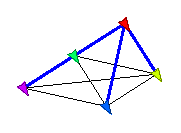
\includegraphics[width=.9\columnwidth]{figs/p-formation}
   \end{minipage}
   \caption{[left] A self-consistent lattice graph for letter ``P''. [right]
     Simulation result of the final formation. 
     The thick blue lines denote the edges in the authority tree.}
   \label{fig:p-letter}
 \end{figure}
 

%\clearpage
\section{Conclusions} 
\label{sec:conc-mrf1}
Above all, we conclude the pros and cons of our algorithm in this chapter.

First, the advantages include:
\begin{enumerate}
\item the algorithm enable multiple robots to form a broad diversity of lattice patterns autonomously with local information;
\item the algorithm runs efficiently and scales reasonably well with increasing numbers of robots;
\item the algorithm is robust to the situation when some robots fail to response others or when more robots join into the system.
\end{enumerate}


However, the major limitations of this primary version include:
\begin{enumerate}
\item the algorithm can not guarantee all the robots eventually reach static positions to form a global lattice pattern, since the lattice graph only reflects local relationships among robots' poses (Figure~\ref{fig:hex-qual});
\item meanwhile, current motion strategy brings side effect on the final formation quality since the orphan robots, who are not assigned any destinations, might move to a position isolated with others.
\end{enumerate}

In the next chapter, we have designed another decentralized formation algorithm to solve these limitations, so that robots can form the desired global patterns in bounded time. Meanwhile, the lattice formation quality is improved.